\documentclass[a4, english]{article}

%Import from a relative path
\usepackage{import}
\import{../../LaTeX-Preamble/}{preamble_dk.tex}
\usepackage{float}

\newcommand*\circled[1]{\tikz[baseline=(char.base)]{
            \node[shape=circle,draw,inner sep=2pt] (char) {#1};}}

\settitle{Eksamensnoter}{Softwarekonstruktion og -arkitektur}
\addauth{Martin Nørskov Jensen}{201610882@post.au.dk}{\, au553262}

\begin{document}

\maketitle

\newpage    
\tableofcontents
\newpage

\section{Test-driven development}
\begin{itemize}
  \item Test-driven development er en del af ekstrem programmering
  \begin{itemize}
    \item En af de første agile metoder 
    \begin{itemize}
      \item Ser software development som en team indsats 
      \item Fokuserer meget på samarbejde med brugerene 
      \item Fokuserer mere på at skrive høj kvalitets kode end at skrive dokumentation
    \end{itemize}
    \item Automatiseret testing er en vigtig del 
    \item Par programmering, hvor person sidder ved computeren og en anden person evaluere koden er central
  \end{itemize}
  \item Alt TDD test produktionskode kommer fra test
  \item Er en iterativ process, hvor man følger TDD rhythm i hver iteration
  \begin{itemize}
    \item Man kan ikke skrive en enkelt linje kode uden at der er en test case, som kræver det
  \end{itemize}
  \item En test liste bruges til at skrive mangle test og tilføje nye test mens koden skrives
\end{itemize}


\subsection{TDD rhythm}
\begin{enumerate}
  \item Quickly add a test
  \item Run all tests and see the new one fail
  \item Make a little change
  \item Run all tests and see them all succeed 
  \item Refactor to remove duplication
\end{enumerate}

\subsection{Values}
\begin{itemize}
  \item Take small steps
  \begin{itemize}
      \item Da hvis man hopper over flere trin, kan man det medfører mange problemer.
      \item Selv hvis det betyder, at man skal skrive midlertidig kode.
  \end{itemize}
  \item Keep focus 
  \begin{itemize}
      \item Fokusere på et trin, et problem ad gangen
  \end{itemize}
  \item Speed 
  \begin{itemize}
      \item at have en velstruktureret programmeringsprocess der bliver guidet fornuftige principper  
      \item test idéer tidligt
      \item at holde koden maintainable og af høj kvalitet 
  \end{itemize}
  \item Simplicity
  \begin{itemize}
      \item implementere kode der får produktet til at virke og ikke mere 
  \end{itemize}
\end{itemize}

\subsection{Principles}
\begin{itemize}
  \item Automated test
  \begin{itemize}
    \item use automated test to test your software
  \end{itemize}
  \item Test First
  \begin{itemize}
    \item Write your test before your write the code that should be tested
  \end{itemize}
  \item Test List
  \begin{itemize}
    \item Before you begin, write a list of all the tests you know you will have to write and add more later
  \end{itemize}
  \item One Steps Test
  \begin{itemize}
    \item Pick a test that will teach you something and that you can implement
  \end{itemize}
  \item Fake It (Til You Make It)
  \begin{itemize}
    \item What is your first implementation once you have a broken test? Return a constant and then gradually transform it 
  \end{itemize}
  \item Triangulation
  \begin{itemize}
    \item Abstract only when you have two or more examples
  \end{itemize}
  \item Isolated Test
  \begin{itemize}
    \item The running of tests should not affect one another
  \end{itemize}
  \item Evident Data
  \begin{itemize}
    \item Make the expected and actual results relationship apparent.
  \end{itemize}
  \item Representative Data
  \begin{itemize}
    \item Select a small set of data where each element represents a conceptual aspect or a special computational processing
  \end{itemize}
  \item Assert First
  \begin{itemize}
    \item Write asserts first
  \end{itemize}
  \item Obvious Implementation
  \begin{itemize}
    \item Just implement simple operations
  \end{itemize}
  \item Evident Tests
  \begin{itemize}
    \item To avoid writing defective tests, we keep the testing code evident, readable and as simple as possible
  \end{itemize}
  \item Child Test
  \begin{itemize}
  	\item If a test case turns out to be too big write smaller test cases that are part of the bigger test case and parses, then reintroduce the larger test case
  \end{itemize}
  \item Do Over
  \begin{itemize}
  	\item When feeling lost, throw away code and start over
  \end{itemize}
  \item Regression Test 
  \begin{itemize}
  	\item When a defect is reported write the smallest test that fails and ones running will be repaired 
  \end{itemize}
  \item Break
  \begin{itemize}
    \item When you feel tired or stuck, take a break,
  \end{itemize}
\end{itemize}

\subsection{Testing terminology}
\begin{itemize}
  \item En \textbf{defekt} (eller bug) er en aritmetisk fejl
  \item En \textbf{test case} er en definition af input værdier og forventede output værdier for et unit under test
  \item En \textbf{test suite} er et set af test cases (ofte repræsenteret af et test case table)
  \item En fejlet test bliver refereret til som en \textbf{broken test}
  \item \textbf{Manuel testing} er hvor test suites bliver eksekveret af mennesker 
  \item \textbf{Automated testing} er en proces hvor test suiten bliver eksekveret af computer og verificeret af mennesker
  \item \textbf{Produktionskode} er kode der defineret softwaren
  \item \textbf{Testkode} er kode der defineret test case for produktionskoden
\end{itemize} 
\begin{figure}[H]
	\centering
	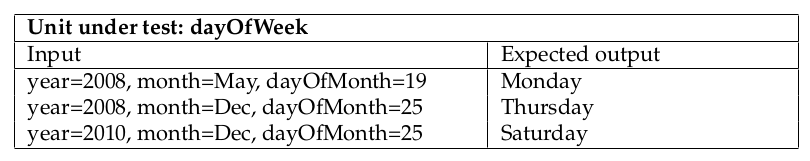
\includegraphics[width=\linewidth]{img/test_case_table_tdd}
	\caption{Test case table	\label{testCaseTableTDDc}}
\end{figure}
\newpage


\section{Systematic black-box testing}
\begin{itemize}
  \item \textbf{Systematisk testing} er en planlagt og systematisk process med et eksplicit mål, som er at finde fejl i en fejldefineret del af systemet 
  \item \textbf{Black-box testing}: unit-under-test bliver behandlet som en sort box
  \begin{itemize}
    \item Den eneste viden man har til at guide testene er specifikationen af UUT, generale  programmeringstekniker samt typisk programmeringsfejl  
  \end{itemize}
  \item \textbf{White-box testing:} hele implementationen er kendt og kan blive brugt til at generer test cases
  \item Der er følgende test-metoder baseret på kompleksiteten af UUT
  \begin{itemize}
    \item \textbf{Ingen testing:} Mange metoder er så små, at de ikke er værd at test
    \begin{itemize}
      \item Fx. assessor metoder
    \end{itemize}
    \item \textbf{Eksplorativ testing:} baseret på erfaring, men følger ikke nogen rigid metode 
    \begin{itemize}
      \item passere bedst til metoder af mellem kompleksitet 
      \item koster lidt 
      \item bliver brugt i TDD
    \end{itemize}
    \item \textbf{Systematisk testing:} her følges en rigid metode til at generer test cases
    \begin{itemize} 
      \item bekostlig, da en del arbejde bliver investeret i analyse af problemet
      \item passer bedst til metoder af høj kompleksitet, hvor tiden brugt giver umagen værd
    \end{itemize}
  \end{itemize} 
\end{itemize}

\subsection{Equivalence class partitioning}
\begin{itemize}
	\item En \textbf{ækvivalens klasse} er et delsæt af alle mulig værdier for UUTen, som har den egenskab at hvis et element demonstrere en defekt i testing, så er det antaget at alle andre værdier producere samme defekt. 
  \item Når man partitioner input element til ECer to egenskaber skal være korrekt for at partitioneringen er sound
  \begin{itemize}
  	\item \textbf{Coverage:} Alle mulige input tilhører mindst en af ækvivalensklasserne 
    \item \textbf{Representation:} Hvis en defekt er demonstreret af en element af en ækvivalensklasse, så er antaget den samme defekt kan blive demonstreret af et hvilket som helst andet element i ækvivalensklassen 
  \end{itemize}
  \item En \textbf{invalid EC} er et defineret til at være et input, der får algoritmen til at bail ud hurtigt 
  \item \textbf{Boundry value analysis}, når man kigger på værdierne der ligger på kanten af en ækvivalensklasserne
  \begin{itemize}
  	\item bruges til at undgå of by one fejl
    \item disse værdier er ofte smarte at bruge i test cases
  \end{itemize}
\end{itemize}

\subsubsection{Partitioning heuristics}
\begin{itemize} 
  \item Lad vær med at generer test cases til inputs der ikke opfylder en precondition
  \item Givet en betingelse, det første set af ECer kan blive udledt ved hjælp af følgende retningslinjer 
  \begin{itemize}
    \item \textbf{Range:} Hvis en betingelse er specificeret for en interval 
    \begin{itemize}
      \item Definer en valid EC dækker intervallet og to invalid en over intervallet og en under
    \end{itemize}
    \item \textbf{Set:} Hvis en betingelse er specificeret for et sæt af værdier
    \begin{itemize}
      \item Definer en EC for hver værdi i sættet og en for alle værdier uden for sættet
    \end{itemize}
    \item \textbf{Boolean:} Hvis en betingelse er specificeret som en skal være betingelse
    \begin{itemize}
      \item Definer en EC for true og en for false
    \end{itemize}
  \end{itemize}
  \item Givet at specifikationen af UUT defineret en aritmetisk operation, så 
  \begin{itemize}
    \item \textbf{Addition og subtraktion:} hvis computeringen indeholder addition eller subtraktion
    \begin{itemize}
      \item Vælg en valid EC for det neutrale element 0 og en valid EC for alle andre elementer 
    \end{itemize} 
    \item \textbf{Multiplikation og division:} hvis computeringen indeholder multiplikation eller division
    \begin{itemize}
      \item Vælg en valid EC for det neutrale element 1 og en valid EC for alle andre 
    \end{itemize} 
  \end{itemize}  
  \item Heuristikkerne for aritmetiske operation, skal bruges på alle elementerne i en computeringen
\end{itemize}

\subsubsection{Myers heuristics}
\begin{itemize}
  \item For at begrænse antallet af test cases \textbf{Myers heuristikkerne} kan blive brugt
  \begin{enumerate}
  	\item Indtil alle valid ECer er dækket, definere en test case, som dækker så mange valide ECer som muligt
    \item Indtil alle invalide ECer er dækkes, definere en test case som kun ligger i en invalid ECn
  \end{enumerate}
  \item For beregninger definere test cases  der kun indeholder ECer med ikke-neutrale elementer
\end{itemize}

\subsubsection{Processen}
\begin{enumerate}
  \item Gennemgå kravene for UUTen og identificere betingelser og brug heuristikker til at finde ECer for hver betingelse
  \item Gennemgå de produceret ECer og overvej repræsentationsegenskaben for elementerne i hver EC
  \begin{itemize}
    \item Hvis man er i tvivl om nogle af elementerne er repræsentative for ECen, så reparationerne ECen
    \item Brug en EC tabel til dette
  \end{itemize}
  \item Gennemgå de produceret ECer for at verificeret at coverage egenskaben er opfyldt 
  \item Generer test case fra ECerne
  \begin{itemize}
    \item Brug Myyers heuristikker for at generer et minimalt sæt af test cases
    \item Brug et test case table til dette 
  \end{itemize}
\end{enumerate}

\subsection{Examples of equivalence class and testcase tables}
\begin{figure}[H]
	\centering
	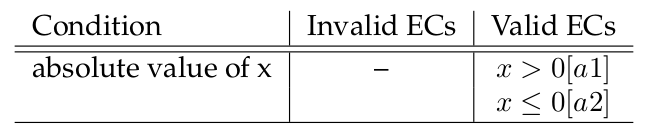
\includegraphics[width=200px]{img/equivalence_table}
	\caption{Ækvivalensklasse tabel	\label{equivalenceClassTable}}
\end{figure}

\begin{figure}[H]
	\centering
	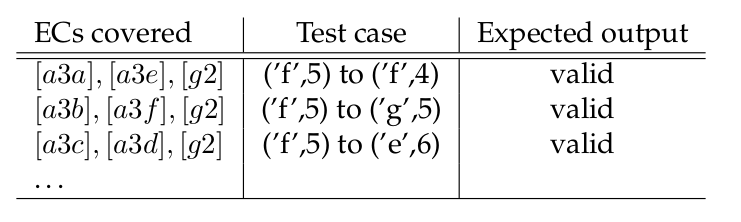
\includegraphics[width=200px]{img/test_case_table}
	\caption{Test case tabel	\label{testCaseTable}}
\end{figure}
\newpage


\section{Variability management}
\begin{itemize}
	\item A \textbf{variability point} er en veldefineret del af produktionskoden, hvis opførelse det skal være muligt at variere  
  \item \circled{3}\circled{1}\circled{2} \ metoden 
  \begin{itemize}
  	\item[\circled{3}] Identificere noget adfærd hvad der varierer  
  	\item[\circled{1}] Definer et ansvar der dækker, denne adfærd
  	\item[\circled{2}] Deleger dette ansvar til en delegate
  \end{itemize}
  \item \textbf{Change by addition:} er adfærd ændringer, der er introduceret ved at tilføje kode uden at ændre i eksisterende produktionskode. 
  \item \textbf{Change by modification:} er adfærd ændringer, der er introduceret ved at modificere eksisterende produktionskode 
  \item \textbf{Open/closed principle:} siger at software skal være åben for udvidelse og lukkede for modifikation
\end{itemize}

\subsection{Source tree copy solution}
\begin{itemize}
	\item En kopi af den original taget til den nye source kode og det der variere ændres i dette 
  \begin{itemize}
  	\item Bliver kaldet \textbf{cut'n'paste reuse}, når man ændre kopier kode for ændre en del af det
  \end{itemize}
  \item Fordele:
  \begin{itemize}
  	\item \textbf{Hastighed:} Det er hurtigt, der skal kun bruges en enkelt kopieringsoperation, samt modificering i testkoden 
    \item \textbf{Simpelt:} Idéen er simpel og hurtig og nem at forklarer til nye programmøre 
    \item \textbf{Ingen implementation indblanding:} To implementation har igen indflydelse på hinanden 
  \end{itemize}
  \item Ulemper:
  \begin{itemize}
  	\item \textbf{Multiple maintenance problem:} Der er flere kode baser at vedligeholde. Hvis en bug er opdaget i den fælles kode, skal den rettes i begge kodebaser 
  \end{itemize}
\end{itemize}

\subsection{Parametric solution}
\begin{itemize}
	\item Et if statement bliver brugt til at vælge hvilken blok af kode, der skal eksekveres baseret på hvilken variation der kører 
  \item Fordele:
  \begin{itemize}
  	\item \textbf{Simpelt:} Conditionals er nemme at forstå og er derfor nemme at beskrive til nye programmøre 
    \item \textbf{Multiple maintenance problemet bliver undgået:} Der er kun en kode base at vedligeholde, derfor er bug fixing meget billigere og fejl er mindre sandsynlige. 
  \end{itemize}
  \item Ulemper:
  \begin{itemize}
  	\item \textbf{Pålidelighedsbekymring:} Nye krav er håndteret ved brug af \textit{change by modification}, hvilket øget riskoen for nye fejl
    \item \textbf{Analysability bekymring:} Når flere og flere krav bliver håndteret ved brug af den parametriske løsning, bliver koden svære at analysere (code bloat)
    \item \textbf{Ansvars erosion:} Klassen får ekstra ansvar i at håndtere de forskellige versioner
  \end{itemize}
\end{itemize}

\subsection{Polymorphic solution}
\begin{itemize}
	\item Subclassing bilver brugt til at lave ny variation af koden
  \item Fordele:
  \begin{itemize}
  	\item \textbf{Multiple maintenance problemet bliver undgået:} der er kun en kode base
    \item \textbf{Pålidelighedsbekymring:} Nye krav bliver håndteret ved brug af \textit{change by addition}
    \item \textbf{Kodes analysability:} Dette forslag gør ikke at koden bliver bloated
  \end{itemize}
  \item Ulemper: 
  \begin{itemize}
  	\item \textbf{Stigende antal klasser:} Nye krav til introducere en ny subklasse
    \item \textbf{Nedarvningsrelationen bliver brugt til en enkelt type af variation:} Man kan ikke bruge nedarvningsrelationen til at håndtere andre typer relationer
    \item \textbf{Genbrug mellem varianter er svært:} Det er svært at bruge algoritmer defineret i en variant i en anden
    \item \textbf{Compile-time binding:} Binding mellem en bestemt variant og klassen bliver bestemt, når koden kompileres.
  \end{itemize}
\end{itemize}

\subsection{Compositional solution}
\begin{itemize}
	\item Variabilitetspunktet bliver delegeret ud til et andet objekt og klassen og dette objekt samarbejde om at fuldføre opgaven
  \begin{itemize}
  	\item Den varierende del bliver indkapslet i et interface 
  \end{itemize}
  \item Fordele:
  \begin{itemize}
  	\item \textbf{Reliability:} Den originale kode bliver refaktoreret til at tage højde for variationen and nye variation af dette variantions punkt kan blive håndteret ved at lave nye klasser
    \item \textbf{Run-time binding:} Bindingen mellem klassen og variationen kan blive ændre på run-time
    \item \textbf{Separation af ansvar:} Ansvar er tydeligt adskilt og tildelt til nemt identificerbar abstraktioner i designet
    \item \textbf{Separation af test:} Variationer kan testes separeret fra hovedklassen.
    \item \textbf{Variations udvælgelse er lokaliseret:} Koden der afgøre hvilken variation, der skal bruges er kun et sted i koden. 
    \item \textbf{Kombinatorisk:} Nye typer af variation kan tilføjes uden at det får indflydelse på eksisterende 
  \end{itemize}
  \item Ulemper:
  \begin{itemize}
  	\item \textbf{Stigende antal klasser og interfaces:} Antallet af klasser og interfaces stiger
    \item \textbf{Klienter må opmærksom på strategierne:} Variant udvælgelse er rykket til klient objekterne 
  \end{itemize}
\end{itemize}

\newpage

\section{Test stubs and unit/integration testing}
\begin{itemize}
	\item \textbf{Direct input:} er de værdier eller data givet af test koden direkte, som har en effekt på opførelsen af unit under test (UUT)
  \item \textbf{Indirect input:} er de værdier eller data, der ikke kan blive givet direkte af test koden, som har en effekt på opførelsen af UUT
  \item \textbf{Depended-On unit (DOU):} et unit i produktionskoden, der giver værdier eller opførsel som har en effekt på UUT
  \item Test double typer (Meszaros (2007))
  \begin{itemize}
    \item \textbf{Test stub:} En double, som er en erstatning af DOU og giver indirekte input, der er defineret af test koden til UUT.
    \begin{itemize}
      \item Test stubbe gøre koden testbar, da de erstatter DOU og gør at test koden kan kontrollere indirekte input. 
    \end{itemize}
    \item \textbf{Test spy:} En double, som skal gemme UUT'ens indirekte input, til senere bekræftelse af test casen.
    \item \textbf{Mock object:} En double, der er skabt og programmeret dynamisk af et mock bibliotek, der både må fungere som en stub og en spy  
    \begin{itemize}
    	\item Man undgår at skrive test stub
      \item Skal fortælles hvad den skal returnerer og i hvilken rækkefølge metoder skal kaldes
      \item Kan være meget besværlige at programmere 
      \item Fejler hurtigt, på den første fejl i protokollen 
    \end{itemize}
    \item \textbf{Fake object:} En double, hvis formål det er erstatte en krævende og dyr DOU 
    \begin{itemize}
    	\item bliver ofte brugt til at erstatte en database 
    \end{itemize}
  \end{itemize}
  \item Der er tre niveauer af testing:
  \begin{itemize}
  	\item \textbf{Unit test:} er processen, hvor man eksekvere software i isolation for at finde defekter 
    \item \textbf{Integrationstest:} er processen, hvor eksekvere software, som samarbejder får at finde fejl defekter i deres interaktion 
    \item \textbf{System test:} er processen, hvor man eksekvere et helt software system for at finde afvigelser fra dens krav
  \end{itemize}
\end{itemize}
\newpage

\section{Design patterns}
\begin{itemize}
	\item Definitioner af design mønster
  \begin{itemize}
  	\item \textbf{Gamma et al. :} Et design mønster er en beskrivelse af kommunikerende objekter og klasser, som er blevet designet til at løse et generalt design problem i en bestemt kontekst.
    \item \textbf{Beck et al. :} Et design mønster er bestemt prosa form af at gemme design information, så at designs der har fungerede godt i fortiden kan bruges i fremtiden. 
    \item \textbf{Role view: } Et design mønster er defineret af et set af roller, som har et specifikt set af ansvar og en veldefineret protokol mellem disse roller
    \item \textbf{Roadmap view:} Design mønster strukturere, dokumentere og giver et overblik over roller og protokoller i komplekse, kompositionel designs. Et design mønster fungere, som en plan (roadmap) af en del af designet. 
  \end{itemize}
  \item \textbf{Rule of three: } En løsning skal være set mindst tre gang i tre forskellige systemer får at kunne betragtes som et mønster 
  \item \textit{Objekt samarbejde definerer kompositionel designs:} Derfor betyder det at når man designer software kompositionel, får de objekter til at samarbejde får at få komplekst opførelse
  \item \textit{Design mønstre er defineret af de problemer de løser: } Det er et problems kendetegn, et design mønster har til formål at løse. 
\end{itemize}
  
\subsection{Compositional design principles}
\begin{itemize}
  \item[\circled{1}] Programmer til et interface, ikke en implementation
  \begin{itemize}
    \item Klienterne kan frit bruge en hvilken som helst service udbyder klasse (lav kobling)
    \item Interfaces giver en mere \textit{fine grained} adfærd abstraktioner, fx. \texttt{Comparable} interfacet
    \item Interfaces udtrykker roller bedre, fx. \texttt{Comparable} interfacet
    \item Klasser definere implementation, såvel som et interface 
  \end{itemize}
  \item[\circled{2}] Foretræk objekt kompostion over klasse nedarvning
  \begin{itemize}
    \item Indkapsling: Klasse nedarvning ødelægger klassen indkapsling og skaber en høj kobling, hvor imod interface giver en god indkapsling samt en lav kobling
    \item Man kan kun tilføje ansvar til klassen, når man bruger nedarvning, ikke fjerne ansvar
    \item Man kan ændre opførelse på run-time ved brug af kompositionel designs, hvor imod nedarvning skal det gøres på compile-time
    \item Klasse hierarkier bliver ofte ændret
    \item Separat testing: Objekt kompostion gør det nemmere at teste forskellig software units i isolation (unit testing)
    \item Bedre mulighed for genbrug
    \item Antallet af klasser, når man bruger objekt komposition stiger og derfor er det vigtigt at have et overblik over klasserne
    \item Delegation giver mere boilerplate kode
  \end{itemize}
  \item[\circled{3}] Overvej hvad der variere i dit design (eller Indkapsle det der variere)
  \begin{itemize}
    \item Forekommer i mange design mønstre fx. \texttt{STRATEGY}
  \end{itemize}
\end{itemize}
\subsection{Design patterns explanation}
\begin{itemize}
	\item \texttt{Strategy}
  \begin{itemize}
  	\item Bruges når man skal understøtte varierende algoritmer eller regler
    \item Algoritmen ansvar bliver givet i et interface, som implementationer af algoritmen implementere
  \end{itemize}
  \item \texttt{State}
  \begin{itemize}
  	\item Bruges når man skal understøtte skiftende algoritmer, når objektets indre tilstand ændre
    \item Konteksten har et tilstandsobjekt for hver tilstand.
    \item Konteksten afgøre hvilket tilstandobjekt den skal kalde afhængig af tilstanden 
  \end{itemize}
  \item \texttt{Abstract Factory}  
  \begin{itemize}
  	\item Bruges når man har en familie af relateret produkter der skal instantiereres på bestemte måder
    \item Gøres ved at lave en abstraktion, hvis ansvar det er at lave familier af objekter.
    \item Objektet delagere objekt oprettelse til dette objekt 
  \end{itemize}
  \item \texttt{Facade}
  \begin{itemize}
	  \item Bruges når kompleksiteten af subsystemet ikke skal vises for klienterne
    \item Gøres ved at definere et interface, der giver simpelt adgang til det komplekse subsystem 
    \item Klienter der bruges subsystemet skal ikke have adgang til det direkte 
  \end{itemize}
  \item \texttt{Decorator}
  \begin{itemize}
  	\item Bruges når man vil tilføje ansvar og opførsel til individuelle objekter under at ændre i klassen
    \item Gøres ved at lave et objekt der implementere det samme interface.
    \item Delagere metode kaldene videre til det rigtige objekt og tilføjer noget opførsel i nogle af metoderne
  \end{itemize}
  \item \texttt{Proxy}
  \begin{itemize}
  	\item Bruges når læsning af objektet er krævene og man derfor først vil loade billedet når det er klart eller når man vil styrer klienters adgang til objektet så som logging, login eller pay-by-access.  
  \end{itemize}
  \item \texttt{Builder}
  \begin{itemize}
  	\item Bruges når man har en bestemt måde at konstruere et objekt på men output formatet variere 
    \item Delagere en del af konstruktionen til et \texttt{Builder} objekt
  \end{itemize}
  \item \texttt{Command}
  \begin{itemize}
  	\item Bruges, hvis man gerne vil konfigurere objekter med opførsel på runtime og/eller understøtte undo
    \item Gøres ved at indkapsle handling i et interface.  
  \end{itemize}
  \item \texttt{Null Object}
  \begin{itemize}
  	\item Bruges i steddet for \texttt{null}, når man gerne vil have et objekt til at gøre ingenting
    \item Gøres ved at definere en implementation af samme interface som objektet der ikke gør noget
  \end{itemize}
  \item \texttt{Adapter}
  \begin{itemize}
  	\item Bruges når man har en klasse med en ønsket funktionalitet, men dens interface og eller protokol svarer ikke overens med det klienten har brug for
    \item Gøres ved at man laver et objekt \texttt{Adapter}, som passer til klientens krav, og som kalder de krævede metoder på en instans af klassen med den ønskede funktionlitet 
    \item \texttt{Adapter} implementere \texttt{Target} interface, som er det interface klienten skal bruge
    \item \texttt{Adaptee} er klassen med den ønskede funktionalitet 
  \end{itemize}
  \item \texttt{Composite}
  \begin{itemize}
  	\item Bruges når man gerne vil håndtere træ datastrukturer
    \item Gøres ved at et fælles interface for \texttt{Leaf} og \texttt{Composite} kaldet \texttt{Component} med delt funktionalitet
    \item \texttt{Composite} har en form for datastruktur med \texttt{Component} typer og deres metoder bliver kaldt med nogle tilføjelser, når metoder bliver kaldt på \texttt{Composite}
  \end{itemize}
  \item \texttt{Observer}
  \begin{itemize}
  	\item Bruges når objekt gerne vil blive notificeret omkring tilstandsændringer på et andet  objekt
    \item Gøres ved at lave et observer interface, som subjektet har en liste af og disse kaldes når den ønskede tilstandsændring kommer
    \item Har to varianter
    \begin{itemize}
    	\item \textbf{Push variant:} subjekt giver besked til observerne med den del af tilstanden der er blevet ændret
      \item \textbf{Pull variant:} subjekt giver besked til observerne uden den del af tilstanden der er blevet ændret 
    \end{itemize}
  \end{itemize}
  \item \texttt{Model-View-Controller}
  \begin{itemize}
  	\item Bruges når man skal understøtte flere vinduer med grafiske brugeflade, der tilgår samme data
    \item \texttt{Model} 
    \begin{itemize}
      \item Gemmer applikationstilstanden
      \item Holder styr på de associerede views
      \item Giver besked til alle views i tilfælde af tilstandsændring
    \end{itemize}
    \item \texttt{View}
    \begin{itemize}
    	\item Visualisere models tilstand grafisk
      \item Acceptere user input og delegere dem til den associerede controller
      \item Hold styr på et sæt af kontrollere og lad brugeren sætte hvilken kontroller er aktiv
    \end{itemize}
    \item \texttt{Controller}
    \begin{itemize}
    	\item Tolke brugerens input og oversæt dem til tilstandændring til modellen 
    \end{itemize}
  \end{itemize}
  \item \texttt{Template-Method}
  \begin{itemize}
  	\item Bruges når man vil have forskellig overførelse i punkter af en algoritme, men algoritmens struktur er den samme
    \item Unification 
    \begin{itemize}
    	\item Både template metoden og hook metoder er inde i den samme klasse
      \item Template metoden er konkret og involvere abstrakte hook metoder der kan bliver overskrevet i en subklasse 
    \end{itemize}
	  \item Seperation
    \begin{itemize}
    	\item Template metoden er defineret i en klasse og hook metoderne er defineret i en eller flere interfaces 
      \item Template metoden er konkret og delegere til implementationer af hook interface(s) 
    \end{itemize}  
  \end{itemize}
\end{itemize}
\newpage

  
\section{Compositional design} 
\begin{itemize}
  \item Definitioner af objekt orientering
  \begin{itemize}
  	\item \textbf{Sprog-specifikke: } Objekter er beholder for metoder og instansvariabler 
    \item \textbf{Model: } Et program ses som en fysisk model der simulere opførelse er en rigtigt en imaginær del af verdenen
    \item \textbf{Ansvars: } Et program er struktureret, som en gruppe af integrerende agenter kaldet objekter, hvor hvert objekt har en rolle og udføre en service eller opgave brugt af de andre medlemmer.
  \end{itemize}
  \item \textbf{Adfærd (behaviour):} at opføre sig på en bestem og observerbar måde
  \item \textbf{Ansvar (responsibility):} Et stadie hvor man bliver ansvarlig og pålidelig for at svare en forespørgsel
  \begin{itemize}
  	\item Skal ikke være for programmeringsspecifik så som at have en \texttt{addPayment} metode
    \item Skal ikke være for åbne og uklare så som \textit{"Opfør sig som en paystation"}
  \end{itemize}
  \item \textbf{Rolle (General):} En funktion eller del som bliver udført i en bestem operation eller proces
  \item Relationen mellem rolle og objekt er en mange til mange relation
  \begin{itemize}
  	\item En rolle kan bliver udført af mange forskellige slags objekter
    \item Et objekt kan have flere roller i et system 
  \end{itemize}
  \item \textbf{Rolle (Software):} Et sæt af ansvar og associerede protokoller
  \item Det er vigtig at definere små og cohesive roller
  \item \textbf{Protokol: } En funktion eller delfunktion der er udført i en bestemt process 
  \begin{itemize}
  	\item Komplekse roller kan defineres ved hjælp af simple roller 
  \end{itemize}
  \item \circled{3}\circled{1}\circled{2} \ metoden 
  \begin{itemize}
  	\item[\circled{3}] Identificere noget adfærd hvad der varierer  
  	\item[\circled{1}] Definer et ansvar der dækker, denne adfærd
  	\item[\circled{2}] Deleger dette ansvar til en delegate
  \end{itemize}
\end{itemize}
\subsection{Compositional design principles}
\begin{itemize}
  \item[\circled{1}] Programmer til et interface, ikke en implementation
  \begin{itemize}
    \item Klienterne kan frit bruge en hvilken som helst service udbyder klasse (lav kobling)
    \item Interfaces giver en mere \textit{fine grained} adfærd abstraktioner, fx. \texttt{Comparable} interfacet
    \item Interfaces udtrykker roller bedre, fx. \texttt{Comparable} interfacet
    \item Klasser definere implementation, såvel som et interface 
  \end{itemize}
  \item[\circled{2}] Foretræk objekt kompostion over klasse nedarvning
  \begin{itemize}
    \item Indkapsling: Klasse nedarvning ødelægger klassen indkapsling og skaber en høj klasser, hvor imod interface giver en god indkapsling samt en høj kobling
    \item Man kan kun tilføje ansvar til klassen, når man bruger nedarvning, ikke fjerne ansvar
    \item Man kan ændre opførelse på run-time ved brug af kompositionel designs, hvor imod nedarvning skal det gøres på compile-time
    \item Klasse hierarkier bliver ofte ændret
    \item Separat testing: Objekt kompostion gør det nemmere at teste forskellig software units i isolation (unit testing)
    \item Bedre mulighed for genbrug
    \item Antallet af klasser, når man bruger objekt komposition stiger og derfor er det vigtigt at have et overblik over klasserne
    \item Delegation giver mere boilerplate kode
  \end{itemize}
  \item[\circled{3}] Overvej hvad der variere i dit design (eller Indkapsle det der variere)
  \begin{itemize}
    \item Forekommer i mange design mønstre fx. \texttt{STRATEGY}
  \end{itemize}
\end{itemize}
\newpage

\section{Frameworks}
\begin{itemize}
	\item Framework kendetegn
  \begin{itemize}
    \item \textbf{Skelet / design / high-level sprog / skabelon}
    \begin{itemize}
      \item Et framework giver applikation adfærd på et høj niveau af abstraktion 
    \end{itemize}
    \item \textbf{Applikation / klasse af software / indenfor et bestemt domæne} 
    \begin{itemize}
      \item Et framework giver en bestemt adfærd i et veldefineret domæne 
    \end{itemize}
    \item \textbf{Samarbejde / samarbejdende klasser}
    \begin{itemize}
      \item Et framework definere protokollen mellem et sæt af veldefineret komponenter / objekter
      \item For at bruge frameworket skal man forestå protokollen
    \end{itemize}
    \item \textbf{Tilpasning / abstrakte klasse / genbruglighed / specialisering} 
    \begin{itemize}
    	\item Et framework er fleksibel, så man kan tilpasse det til en bestem kontekst, så længe at den kontekst er inde i domænet af frameworket 
    \end{itemize}
    \item \textbf{Klasser / implementation / skelet }
    \begin{itemize}
    	\item Et framework er genbrug af kode såvel som design
    \end{itemize}
  \end{itemize}
  \item \textbf{Inversion of control}
  \begin{itemize}
  	\item Frameworket definere the flow of control ikke dig
    \item Bliver ofte beskrevet af Hollywood princippet \textit{"Don't call us we'll call you"}
    \item Modsat et bibliotek 
  \end{itemize}
  \item På grund af Inversion of control egenskaben definere frameworket også 
  \begin{itemize}
  	\item Objekt protokoller
    \item Variabilitets punkter  
  \end{itemize}
  \item \textbf{Software produkt linje: }
  \begin{itemize}
  	\item er et set af software krævende systemer, som deler et fælles set af features
    \item imødekommer de konkrete krav af et bestemt marked, eller mission
    \item er blevet udviklet fra de samme hoved assets på en beskrevet måde
  \end{itemize}
\end{itemize}  
\subsection{Frozen and hot spots}
\begin{itemize}
	\item \textbf{Frozen spot}
  \begin{itemize}
  	\item en del af frameworkets kode som ikke kan blive ændret
    \item definere det basale design og objekt protokoller i den endelige applikation  
  \end{itemize}
  \item \textbf{Hot spot} (hook variability points)
  \begin{itemize}
  	\item en defineret del af frameworket 
    \item specialiseringskode kan ændre eller tilføje adfærd til applikationen 
  \end{itemize}
  \item Frameworkets bliver ikke tilpasset af kode modifikation
  \begin{itemize}
  	\item Frameworks er en lukket sort boks, hvor source koden ikke må blive ændret
    \item Tilpasning må kun ske gennem den givne adfærd i hot spots, af de mekanismer givet af framework programmørene  
    \item Change by addition ikke modification    
  \end{itemize}
  \item Mange frameworks kommer med standard implementationer for de fleste eller alle variabilitetspunkter 
\end{itemize}
\subsection{Defining Variability Points}
\begin{itemize}
  \item \textbf{Framework kode:} Koden der definere frameworket 
  \item \textbf{Applikationskode:} Koden der definere specialiseringen af variabilitetspunkterne  
	\item Et framework skal bruge dependency injection
  \begin{itemize}
  	\item Frameworket selv kan ikke instantierer objekter som definere variabilitetspunkter
    \item Variabilitetspunkterne selv skal blive instantiereret af applikationskoden og injected ind i frameworket 
  \end{itemize}
  \item En regel siger, at framework kode ikke må bruge et \texttt{new} statement på klasser der har hotspot metoder defineret   
  \item Et framework giver en række muligheder for at definere hot spot objekter
  \begin{itemize}
  	\item Eksisterende konkrete klasser 
    \begin{itemize}
    	\item Et framework kommer med en række prædefineret klasser 
      \item Det er applikationsprogrammørens job at lave de prædefineret klasser til noget brugbart
      \item Fx. AWT og swing til GUI
    \end{itemize}
    \item Subklasser og abstrakte klasser
    \begin{itemize}
    	\item Frameworket har abstrakte klasser
      \item Største delen af implementation med høj kvalitet er allerede givet
      \item Udvikleren skal give de sidste detaljer 
    \end{itemize}
    \item Implementation af et interface
    \begin{itemize}
    	\item Frameworket indeholder et interface
      \item Giver applikationsudvikleren muligheden for at have fuld kontrol over hot spots 
    \end{itemize}
  \end{itemize} 
  \item Et framework skal understøtte spekteret fra igen implementation (interface) til delvis (abstrakt) til fuldt (konkret) implementation for variabilitetspunkterne.
\end{itemize}
\subsection{TEMPLATE METHOD}
\begin{itemize}
  \item Unification 
  \begin{itemize}
  	\item Både template metoden og hook metoder er inde i den samme klasse
    \item Template metoden er konkret og involvere abstrakte hook metoder der kan bliver overskrevet i en subklasse 
  \end{itemize}
	\item Seperation
  \begin{itemize}
  	\item Template metoden er defineret i en klasse og hook metoderne er defineret i en eller flere interfaces 
    \item Template metoden er konkret og delegere til implementationer af hook interface(s) 
  \end{itemize}
\end{itemize}

\subsection{Compositional design principles}
\begin{itemize}
  \item[\circled{1}] Programmer til et interface, ikke en implementation
  \begin{itemize}
    \item Klienterne kan frit bruge en hvilken som helst service udbyder klasse (lav kobling)
    \item Interfaces giver en mere \textit{fine grained} adfærd abstraktioner, fx. \texttt{Comparable} interfacet
    \item Interfaces udtrykker roller bedre, fx. \texttt{Comparable} interfacet
    \item Klasser definere implementation, såvel som et interface 
  \end{itemize}
  \item[\circled{2}] Foretræk objekt kompostion over klasse nedarvning
  \begin{itemize}
    \item Indkapsling: Klasse nedarvning ødelægger klassen indkapsling og skaber en høj kobling, hvor imod interface giver en god indkapsling samt en lav kobling
    \item Man kan kun tilføje ansvar til klassen, når man bruger nedarvning, ikke fjerne ansvar
    \item Man kan ændre opførelse på run-time ved brug af kompositionel designs, hvor imod nedarvning skal det gøres på compile-time
    \item Klasse hierarkier bliver ofte ændret
    \item Separat testing: Objekt kompostion gør det nemmere at teste forskellig software units i isolation (unit testing)
    \item Bedre mulighed for genbrug
    \item Antallet af klasser, når man bruger objekt komposition stiger og derfor er det vigtigt at have et overblik over klasserne
    \item Delegation giver mere boilerplate kode
  \end{itemize}
  \item[\circled{3}] Overvej hvad der variere i dit design (eller Indkapsle det der variere)
  \begin{itemize}
    \item Forekommer i mange design mønstre fx. \texttt{STRATEGY}
  \end{itemize}
\end{itemize}


\newpage

\section{Clean Code and Refactoring}
\begin{itemize}
	\item \textbf{Small}
  \begin{itemize}
  	\item Indent niveauet af en funktion må aldrig være mere end en eller to
  \end{itemize}
  \item \textbf{Do One Thing}
  \begin{itemize}
  	\item En funktion skal kun gøre en ting.
  \end{itemize}
  \item \textbf{One Level of Abstraction}
  \begin{itemize}
  	\item En funktion skal bruge det samme niveau af abstraktion
  \end{itemize}
  \item \textbf{Use Descriptive Names}
  \begin{itemize}
  	\item En funktion navn skal tydelig beskrive hvad den ene ting den gør
  \end{itemize}
  \item \textbf{Keep the Number of Arguments Low}
  \begin{itemize}
    \item Færrest muligt argumenter er bedst 
    \item 0-1-2 argumenter måske 3, hvis funktionen bruger flere argumenter gør den mere end en ting
  \end{itemize}
  \item \textbf{Avoid Flags Arguments}
  \begin{itemize}
  	\item Man skal ikke bruge flag argumenter til funktioner, da det betyder at funktionen gør noget forskellige afhængige af flag argumentet 
  \end{itemize}
  \item \textbf{Have No Side Effects}
  \begin{itemize}
  	\item Funktionen skal kun gøre det, den siger den gør.
    \item Det skal altid være sikkert at kalde en funktion.
  \end{itemize}
  \item \textbf{Command Query Separation}
  \begin{itemize}
    \item Accessors and mutators
    \item \textbf{Query:} Ingen state ændring
    \item \textbf{Command:} Ingen retur værdi
  	\item Metoder skal enten give et resultat eller ændre noget i begge ting.
  \end{itemize}
  \item \textbf{Prefer Exceptions to Error Codes}
  \begin{itemize}
  	\item Man skal heller smide en exception end at returnere fejl koder
  \end{itemize}
  \item \textbf{Don't Repeat Yourself}
  \begin{itemize}
  	\item Man skal ikke have det samme kode to gange i ens kode base
    \item For at undgå Multiple maintanance problem
  \end{itemize}
  \item \textbf{Do the Same Thing the Same Way}
  \begin{itemize}
  	\item Man skal gør den samme ting på samme måde
    \item Gør ens kode nemmere at bruge 
  \end{itemize}
  \item \textbf{Name Boolean Expressions}
  \begin{itemize}
  	\item Navngiv Boolean expression, gør koden nemmere at læse 
  \end{itemize}
  \item \textbf{Bail Out Fast}
  \begin{itemize}
  	\item Tjek boolean expression individuelt og returnere \texttt{false}, hvis en fejler
  \end{itemize}
  \item \textbf{Arguments in Argument Lists}
  \begin{itemize}
  	\item Argumenter høre til i argument lister ikke som en del af en funktion
    \item Undgå at et argument er en del af metode navnet fx \texttt{moveUnitForBluePlayer}
  \end{itemize}
\end{itemize}
\subsection{Flexibility and Maintainability}
\begin{figure}[H]
	\centering
	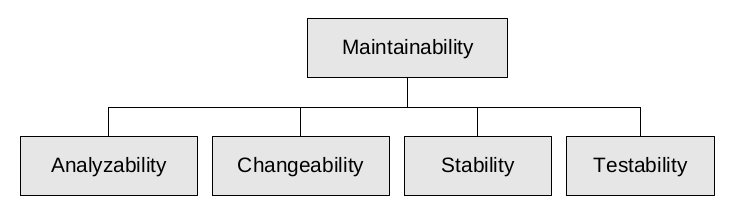
\includegraphics[width=\linewidth]{img/maintain}
\end{figure}
\begin{itemize}
	\item \textbf{Maintainability:} Softwarens evne til at blive ændret
  \begin{itemize}
  	\item Ændringer kan være rettelser, forbedringer, tilpasning til ændringer, krav og funktionelle specifikationer
    \item Kan blive målt i hvor meget det koster at ændre softwaren 
  \end{itemize} 
  \item \textbf{Analysability:} Softwarens evne til blive diagnosticere mangler eller årsagen til fejl
  \begin{itemize}
  	\item Evnen til at forstå softwaren
    \item Det er vigtig at kunne forestå og læse softwaren
  \end{itemize} 
  \item \textbf{Changeability:} Softwarens evne til muligøre specifik modifikation
  \begin{itemize}
  	\item Evnen til at tilføj, ændre og forbedre en feature i et system til en fornuftig pris
    \item Der er to forskellige dele 
    \begin{itemize}
    	\item De aspekter der kan ændres på compile time
      \item De aspekter der kan ændres på runtime
    \end{itemize}
  \end{itemize}
  \item \textbf{Stability:} Softwarens evne til at undgå uforudset effekter fra modifikationer af systemet
  \item \textbf{Testability:} Softwarens evne til at validere et modificeret system
  \begin{itemize}
  	\item Evenen til at teste software
  \end{itemize}
  \item \textbf{Flexibility:} Softwaren evne til at understøtte tilføjet/forbedret funktionalitet udelukkende ved at tilføje software dele
  \begin{itemize}
  	\item Evnen til at tilføje funktionalitet ved at tilføj dele
    \item Et specielt tilfælde af changeability
  \end{itemize}

\end{itemize}

\subsection{Coupling and Cohesion}
\begin{itemize}
	\item \textbf{Kobling:} Det måler hvor meget en software unit afhænger af andre software units 
  \begin{itemize}
  	\item Afhængigheder mellem software kommer i mange former
    \begin{itemize}
    	\item Metoder afhænger af klassen instans variabler
      \item Klasser afhænger af hinanden, når de er refereret i kode 
      \item Mellem pakker
    \end{itemize}
    \item En software enhed kan have en høj eller lav kobling
    \item En høj kobling formindsker maintainability
    \begin{itemize}
    	\item Den formindsker også reliability, da en bug er mere sandsynlig
      \item Koden bliver svære at læse
      \item Det bliver svære at genbruge
    \end{itemize}
    \item En lav kobling gør generelt kode mere pålidelig 
    \begin{itemize}
    	\item Gør koden nemmere at genbruge
    \end{itemize} 
  \end{itemize}
  \item \textbf{Kohæsion:} Det måler hvor meget relateret og fokuseret krav og de givne adfærd i en software unit er.
  \begin{itemize}
  	\item Det betyder om koden er organiseret
    \item En kvalitet, man som udvikler skal gå efter 
    \item En høj kohæsion betyder at software enheder har få tæt relateret krav
    \begin{itemize}
    	\item Hjælper på reliability og maintainability
      \item Forøger analysability
      \item Gør det nemmere at undgå fejl
    \end{itemize}
  \end{itemize}
  \item \textbf{Law of Demeter:} Den siger, at man ikke skal samarbejde med indirekte objekter
  \begin{itemize}
  	\item Bliver også kaldt \textit{"do not talk to strangers"}
    \item I en metode skal man kun kalde metoder på 
    \begin{itemize}
    	\item \texttt{this}
      \item En metodes parameter
      \item En attribut af \texttt{this} 
      \item Et element i en samling hvilken er en attribut af \texttt{this}
      \item Et objekt lavet inden i metoden 
    \end{itemize}
    \item Det er en mere en design regel end lov
    \item Hjælper imod høj kobling 
  \end{itemize}
\end{itemize}
\newpage

\section{Distribution and Broker}
\subsection{Distributed computing}
\begin{itemize}
	\item Distribuerede computing er et felt i Datalogi, der studerer distribuerede systemer
  \item \textbf{Distribuerede system:} Et system, hvor komponenter, lokaliseret på netværk computere, kommunikere og kordinere deres handlinger kun ved passere beskeder 
  \item \textbf{Klient-server arkitektur:}
  \begin{itemize}
  	\item To komponenter har brug for at snakke sammen, og er uafhængige af hinanden.
    \item En af komponenter indikere er forbindelse den anden udbyder
    \item Den komponent der udbyder servicen skal kunne håndter et antal forbindelser på samme tid
    \item Den der anmoder komponent skal kunne håndtere forskellige resultater
  \end{itemize}
  \item CLIENT-SERVER mønsteret skelner mellem to typer komponenter klienter og serverer
  \begin{itemize}
  	\item Klienten anmoder information eller services fra en server hvilket betyder at den skal kende
    \begin{itemize}
    	\item Hvordan man forbinder til serveren, hvilken kræver et id eller en adresse til serveren
      \item Serverens interface
    \end{itemize}
    \item Serveren svarer på klientens request
    \begin{itemize}
    	\item processer hver request for sig selv
      \item kender ikke idet klientens adresse eller id før interaktionen  
    \end{itemize}
    \item Klienter er optimeret til deres applikationsopgave 
    \item Serverer er optimeret til at håndtere flere klienter
  \end{itemize}
  \item \textbf{Request-Reply protocol:} simulere synkron kald mellem klient og server ved parvis udveksling af beskeder
  \begin{itemize}
  	\item En former request beskeden fra klient til serveren
    \item Anden former reply beskeden fra serveren tilbage til klienten
    \item Klienten sender request beskeden for venter/blokere indtil reply besked er blevet modtaget
  \end{itemize}
  \item \textbf{Marshalling:} Det er processen, hvor man tager en kollektion af struktureret data elementer og samler dem til et byte array, som kan bruges til at sende netværks beskeder
  \item \textbf{Unmarshalling:} Det er processen, hvor man laver et byte array modtaget over en netværk besked til en ækvivalent samling af struktureret data elementer.
  \item Marshalling og demarshalling processen skal være enig om formatet, marshalling formatet 
  \item \textbf{Named services:} De kan bliver brugt til at oversætte et navn for et fjern objekt til en konkret location og identitet 
  \begin{itemize}
  	\item Java RMI giver et register hvor man kan binde et navn til en location
    \item DNS servere binder urler så som \texttt{google.dk} til en konkret ip-adresse
  \end{itemize}
\end{itemize}
\subsection{Broker}
\begin{figure}[h!]
	\centering
	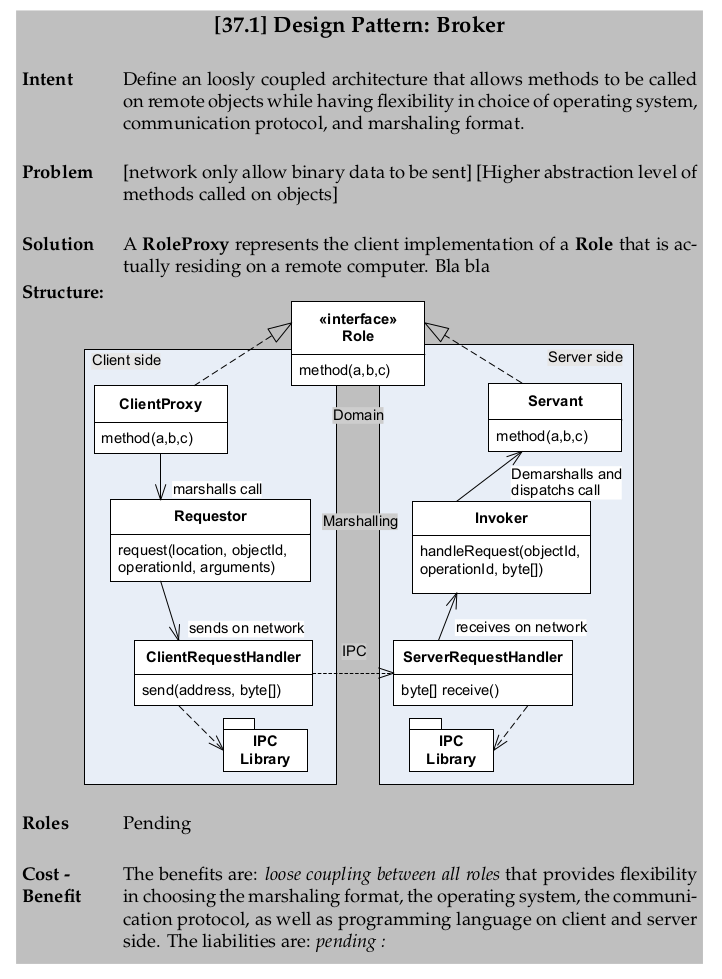
\includegraphics[width=\linewidth]{img/broker_pattern}
\end{figure}
\begin{itemize}
	\item \texttt{ClientProxy}
  \begin{itemize}
  	\item \texttt{PROXY} for remote servant objekt
    \item Implementere det samme interface som \texttt{Servant}
    \item Oversætte alle metoder kald til kald til den associerede \texttt{Reqestor}'s \texttt{request} metode
  \end{itemize}
  \item \texttt{Requestor}
  \begin{itemize}
  	\item Laver mashalling af metode navn og argumenter til et \texttt{RequestObject}
    \item Kalder den associerede \texttt{ClientRequestHandler}'s \texttt{send} metode
    \item Demarshalling returneret \texttt{ReplyObject} til retur værdi(er)
    \item Lav klientside expections, hvis der er sket fejl på server siden 
  \end{itemize}
  \item \texttt{RequestObject}
  \begin{itemize}
  	\item Indkapsler alt information omkring metode kald, inkluderende objekt identitet, server location og parameter i et marshalling format  
  \end{itemize}
  \item \texttt{ClientRequestHandler}
  \begin{itemize}
  	\item Udfører alt \textit{inter process communication} for klientsiden 
  \end{itemize}
  \item \texttt{ServerRequestHandler}
  \begin{itemize}
  	\item Udfører alt \textit{inter process communication} for serversiden 
    \item Indeholder en event loop tråd der venter på request fra netværket 
    \item Når den modtager en besked, kalder den \texttt{Invoker} med det modtagende \texttt{RequestObject}
  \end{itemize}
  \item \texttt{Invoker}
  \begin{itemize}
  	\item Udfører demarshalling af \texttt{RequestObject}er
    \item Afgøre hvilke objekter, metoder, argumenter og kald på den identificeret \texttt{Servant} objekt 
    \item Udfører marshalling af retur værdien fra \texttt{Servant} objektet til et \texttt{ReplyObject}
  \end{itemize}
  \item \texttt{ReplyObject}
  \begin{itemize}
    \item Indkapsler alt information omkring retur værdier, inkluderende exception smidt og fejl 
beskeder, fra metode kald i et marshalling format 
  \end{itemize}
  \item \texttt{Servant}
  \begin{itemize}
  	\item Domæne objekt med domæne implementation på serversiden
  \end{itemize}
  \item \textit{Altid inkludere format versionen, når man bruger marshalling}
\end{itemize}
\subsection{Example implementation}
\begin{itemize}
	\item ClientProxy:
  \begin{lstlisting}[language=java]
  package breakthrough.client;

  public class BreakthroughProxy implements Breakthrough, ClientProxy {
      private Requestor requestor;

      public BreakthroughProxy(Requestor requestor) {
          this.requestor = requestor;
      }

      @Override
      public Color getPieceAt(Position p) {
          return requestor.sendRequestAndAwaitReply(
                  p.toString(),
                  OperationNames.GET_PIECE_AT_OPERATION,
                  Color.class,
                  p
          );
      }

  }
  \end{lstlisting}
  \item Invoker:
  \begin{lstlisting}[language=java]
  package breakthrough.marshall.json;

  public class StandardJSONInvoker implements Invoker {

      private Breakthrough breakthrough;
      private Gson gson;

      public StandardJSONInvoker(Breakthrough breakthrough) {
          this.breakthrough = breakthrough;
          gson = new Gson();
      }

      @Override
      public ReplyObject handleRequest(String objectId, String operationName, String payload) {
          ReplyObject replyObject = null;

          JsonParser parser = new JsonParser();
          JsonArray array = parser.parse(payload).getAsJsonArray();

          switch (operationName){
              case OperationNames.GET_PIECE_AT_OPERATION:
                  Position position = gson.fromJson(array.get(0),Position.class);
                  replyObject = new ReplyObject(
                          HttpServletResponse.SC_OK,
                          gson.toJson(breakthrough.getPieceAt(position))
                  );
                  break;
              case OperationNames.GET_PLAYER_IN_TURN_OPERATION:
                  replyObject = new ReplyObject(
                        HttpServletResponse.SC_OK,
                        gson.toJson(breakthrough.getPlayerInTurn())
                  );
                  break;
              default:
                  replyObject = new ReplyObject(HttpServletResponse.
                          SC_NOT_IMPLEMENTED,
                          "Server received unknown operation name: '"
                                  + operationName + "'.");
                  break;
          }

          return replyObject;
      }
  }
  \end{lstlisting}
\end{itemize} 
\newpage


\end{document}
%%% Local Variables:
%%% mode: latex
%%% TeX-master: t
%%% End:
